\documentclass[../main.tex]{subfiles}
\begin{document}
\chapter{Results}
\label{cha:results}

\section{Overview}  % mention the most important results and briefly explain the next sections 
\label{sec:results_overview}
This section will cover the wide range of results obtained during the research process.
% Perhaps replace the reference to the Dataset chapter with a reference to a more specific section once it is created
All six models mentioned in the earlier sections were trained on six datasets: the five datasets of recordings made using different keyboards and microphones (see Section~\ref{sec:dataset_recorded_datasets} for their description) and an "all" dataset, which combines the remaining five into a single one.
After training, every model was tested using all datasets to gauge its generalization ability.
This procedure was conducted for all three types of preprocessing (raw, FFT, MFCC), and all seven combinations of the three peak types (\peaks{thr}, \peaks{th}, \peaks{tr}, \peaks{hr}, \peaks{t}, \peaks{h}, \peaks{r}).
This configuration leads to 4536 testing procedures (see Equation~\ref{eq:num_tests}): 
%DONE MK do not use caption for the equations; equations can be number \begi{equation} or not \begin{equation*}; when they are numbered, they can be referred by label and ref
\begin{equation}
    \mathrm{Models} \cdot \mathrm{Train} \cdot \mathrm{Test} \cdot \mathrm{PreProc} \cdot \mathrm{PeakComb} = 6 \cdot 6 \cdot 6 \cdot 3 \cdot 7 = 4536.
    \label{eq:num_tests}
\end{equation}
For each of them, a single metric -- accuracy -- is reported. 

The best accuracy attained among all 4536 test runs is \textbf{88.4\%}. It was reached by two models -- SVM and 1-NN, both using MFCC preprocessing, tested on the highest quality dataset (Main).
SVM can reach this value only when it is trained exclusively on the highest quality data, while 1-NN is capable of this feat in this case and when it is trained on the "all" dataset.
The latter suggests that the cleanest dataset is "disjoint" with the rest of the data -- its members are never closer to keystrokes from other recordings than to ones from within itself.

The experiments also made it abundantly clear that it is tough for any simple type of model to successfully classify the keystrokes of a keyboard it had not been trained on. 
In those situations, the results are better than random, reliably exceeding 4\% accuracy -- see Figure~\ref{fig:best_model_per_train_test} (guessing 1 out of 43 keys corresponds to a baseline random-guess accuracy of 2.3\%). 

\begin{figure}[H]
    \centering
    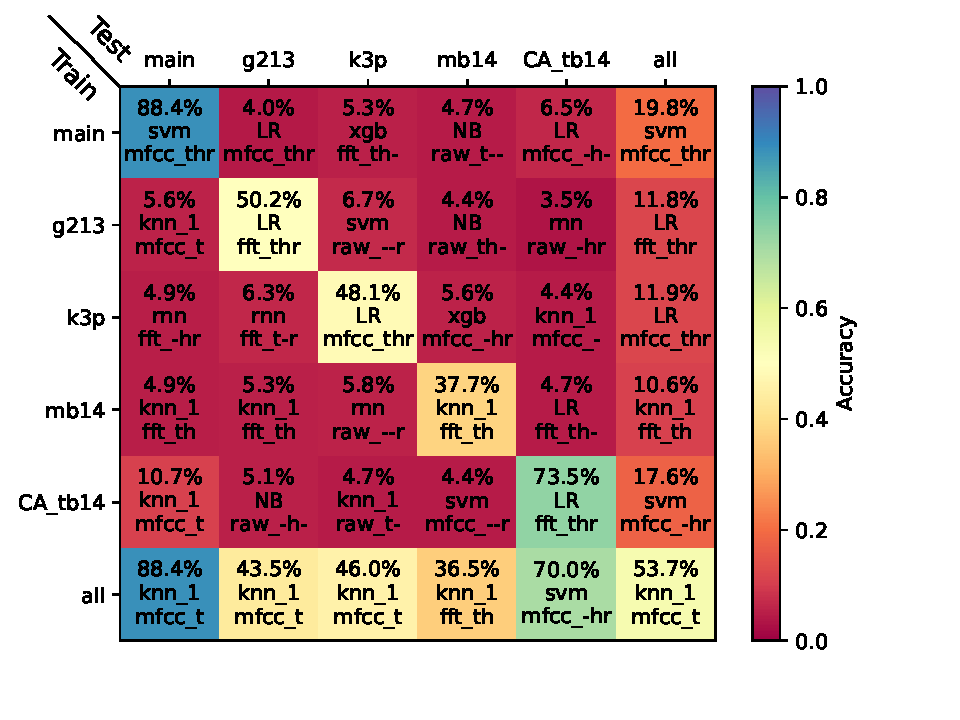
\includegraphics[width=0.8\textwidth]{figures/plots/best_models_per_train_test.pdf}
    \caption{Plot illustrating the best-performing model on each pair (train, test)}
    \label{fig:best_model_per_train_test}
\end{figure}

%DONE MK not "This plot", but "The plot illustrated in Figure~\ref{fig:best_model_per_train_test}; each figure/table needs to be referred in the text
The plot illustrated in Figure~\ref{fig:best_model_per_train_test} also serves as the best visualization supporting the hypothesis that the keyboard used has a more significant impact on a model's predictive ability than the recording microphone (when other factors are assumed to be unchanged).
Models trained on CA\_tb14 could reach significantly higher accuracies when tested on Main (10\% and above) than any model trained on a dataset consisting of one keyboard and tested on another -- the highest accuracy obtained in a configuration like this is 6.7\%. 
The 6.5\% accuracy of a model trained on Main and tested on CA\_tb14 also supports this claim -- it is the highest among the scores for models trained on Main and tested on a different keyboard.
When two datasets used the same microphone but different keyboards (Main, G213, K3P), the best performance when tested on a different dataset does not necessarily come from the other one from within the group -- e.g., when trained on K3P, models did better when tested on MateBook14 than on Main or G213.


% TODO: ensure this is where the full results data is to be found
% DONE MK not "paper", but "thesis"
% DONE? - make sure that this stays on one page; there might be "more correct" way 
\vbox{
All of the raw results that were used to prepare this and the following plots are provided in the .json files made available with the thesis.
The files are in the format:
\begin{verbatim}
{
    training_dataset: {
        testing_dataset : {
            "peak_type1": accuracy,
            "peak_type2": accuracy,
            ...
        },
        ...
    },
    ...
}
\end{verbatim}
}

% DONE: verify that this is the case
A wider variety of plots showcasing the results can be found in Appendix~\ref{cha:plots}. Tables, including all accuracy values for scenarios where models were trained and tested on the same recording configuration, are available in Appendix~\ref{cha:tables}.

%

\section{Best performers per dataset}  % Go over each dataset and how its characteristics might have impacted the results
\label{sec:results_best_performers_per_dataset}
This section will review all the datasets, examining which models performed best on each.
The main takeaway is that different models excel at handling different types of recordings. There is no approach significantly dominating all others when a range of datasets as diverse as discussed here is concerned.
Most of the analysis will be based on examining the top 20 results across all test runs on a given dataset.
% consider some standardization: maybe always include the model types and preprocessing counts? 
%
\subsection{Main}
The Main dataset, being the one with the most deliberate recordings, was the one with by far the best performances across the board. Accuracy of 80\% was exceeded 16 times (no model could cross this threshold on any other dataset, and only 6 exceeded 70\% on CA\_tb14). 
1-NN, SVM, Logistic Regression, and RNN are the model types capable of crossing this threshold (in order of non-increasing accuracy). 
Among the top 20 performances, FFT or MFCC was always used (12 and 8 times, respectively); all twenty accuracies can be examined in Figure~\ref{fig:best_acc_per_dataset_main}.

Preprocessing techniques: 0, 12, 8 (raw, FFT, MFCC).
Best performer: 1-NN and SVM, MFCC, \peaks{thr}: 88.4\% accuracy (tie -- result of getting 380/430 test cases correctly).

\begin{figure}[H]
    \centering
    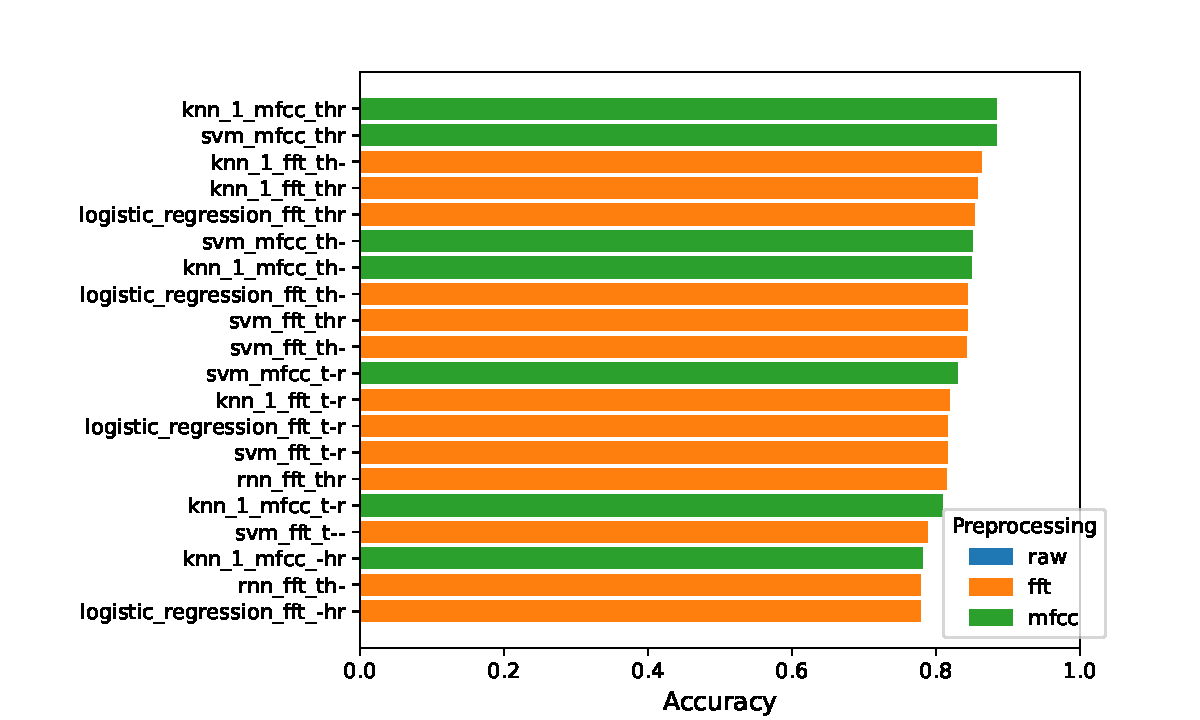
\includegraphics[width=0.8\textwidth]{figures/plots/best_acc_per_dataset/main_dataset.pdf}
    \caption{The 20 highest accuracies achieved on the Main dataset}
    \label{fig:best_acc_per_dataset_main}
\end{figure}

%
\subsection{G213}
No other dataset has such a clear single type of model dominating the top of the ranking. The four highest accuracies (50.2\%--45.3\%) were achieved by Logistic Regression models, all including the touch peak (in order of accuracy, highest to lowest: \peaks{thr}, \peaks{th}, \peaks{tr}, \peaks{t}). What is also unique about G213 is that in the top 20, the touch peak is always included -- for all other datasets, there is at least one case when it is omitted. This suggests that for this keyboard, the earliest parts of keystroke sounds are particularly characteristic for each key.

Preprocessing techniques: 2, 9, 9 (raw, FFT, MFCC).
Best performer: Logistic Regression, FFT, \peaks{thr}: 50.2\% accuracy.
%

\subsection{K3P}
\label{sec:results_K3P}
While there was a strong preference towards a type of model in the previous dataset, for K3P, there is a preference towards a type of preprocessing -- 17 of the 20 best accuracies (and the entire top 8) were achieved with the use of MFCC (the remaining 3 with FFT). This was also the dataset in which XGBoost performed the best relative to its peers - achieving rank 13 (accuracy 36.3\%, MFCC, \peaks{thr}), and 2 more top 20 placements. 

Preprocessing techniques: 0, 3, 17 (raw, FFT, MFCC).
Best performer: Logistic Regression, MFCC, \peaks{thr}: 48.1\% accuracy.
%
\subsection{MateBook14}
This is the only dataset for which the accuracy threshold of 40\% was never exceeded (highest: 37.7\%).
This was also the only time that Naive Bayes cracked the top 10, doing it just barely at the 10th spot, using \peaks{th} and MFCC to reach an accuracy of 30.9\%. 

Preprocessing techniques: 4, 8, 8 (raw, FFT, MFCC).
Best performer: 1-NN, FFT, \peaks{thr}: 37.7\% accuracy.
%
\subsection{CA\_tb14}
\label{sec:results_CA_tb14}
The second dataset recorded on the loudest keyboard, and the one where RNN performed the best relative to its competitors, with two top 5 appearances. 
One peculiarity of results on this dataset is the surprisingly good performance of models using only the \peaks{hr} peaks -- it occurred seven times within the top 20 (see Figure~\ref{fig:best_acc_per_dataset_CA_tb14}), including the 2nd and 3rd spots. 
% additional comment by BW
Another quite exceptional thing is that \peaks{t} conveys much less information here than when compared to other datasets. In almost all other cases, regardless of preprocessing \peaks{h} and \peaks{r} were inferior to \peaks{t}. What is more, \peaks{h} and \peaks{r} achieve similar results to \peaks{th} and \peaks{tr}, further reinforcing that \peaks{t} provides little to no value for chosen models. 
It is, however, still impactful, as its addition is what differentiates the second best and the best performer. 

Preprocessing techniques: 0, 11, 9 (raw, FFT, MFCC).
Best performer: Logistic Regression, FFT, \peaks{thr}: 73.5\% accuracy.

\begin{figure}[H]
    \centering
    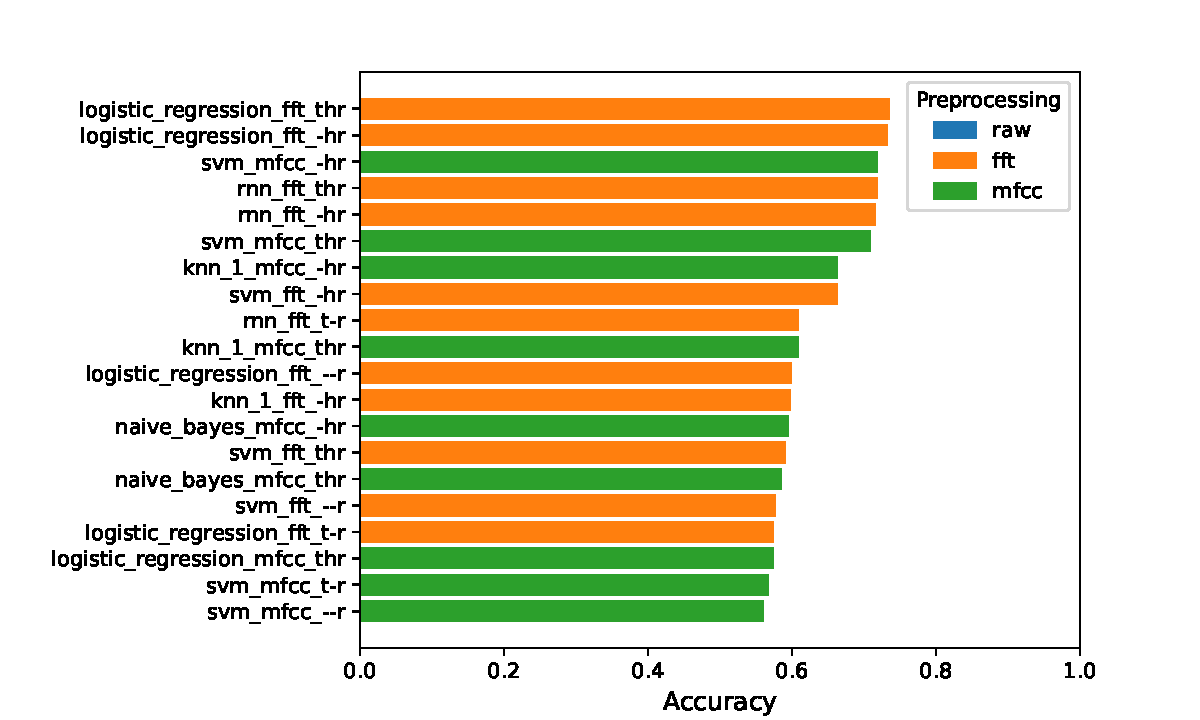
\includegraphics[width=0.8\textwidth]{figures/plots/best_acc_per_dataset/CA_tb14_dataset.pdf}
    \caption{The 20 highest accuracies achieved on the CA\_tb14 dataset}
    \label{fig:best_acc_per_dataset_CA_tb14}
\end{figure}

%
\subsection{All}
For the most diverse dataset, 1-NN  performed surprisingly well -- it claimed 14 spots within the top 20. 
This might be due to learning any particular properties on such a general scale is challenging, and the local information gained by identifying the closest neighbor retains its value. 
It also boasted by far the largest discrepancy between 1st and 2nd highest accuracies: 4.7 percentage points (the 2nd, 49.0\% was reached by SVM, MFCC, \peaks{thr})

Preprocessing techniques: 5, 5, 10 (raw, FFT, MFCC).
Best performer: 1-NN, MFCC, \peaks{thr}: 53.7\% accuracy.

% DONE PK: redact (this is the first section ever written by me and it's never been updated)
\section{Model comparisons}
\label{sec:results_model_comparison}
This section will focus on comparing the performances of all models across all datasets and preprocessing types. To keep things simple, only configurations using \peaks{thr} will be considered. This is because every model type in this thesis achieved its best accuracy on data comprising all three peak types.

All models behave slightly differently, but some correlations are worth highlighting. Whether these correlations tell some truth about the nature of the models used or are plain coincidences is not easily determinable, and further analysis of this kind is not the goal of this thesis.

\subsection{Similar responses to preprocessing}
Some models seem to share the same \emph{preprocessing rankings} when given the same dataset. A preprocessing ranking of a model is defined as a best-to-worst ordering of preprocessing techniques with respect to how well the given model performed using each of them. In other words, a group of such models will (almost) always have the same preprocessing ranking, even if they vary across datasets.

\subsubsection{1-NN, XGBoost, SVM}
This kind of relationship was most notably observed for 1-NN, XGBoost, and SVM. These models shared the same preprocessing ranking on 4 out of 6 datasets (Figure~\ref{fig:selective_model_comparison_knn_xgboost_svm_main} illustrates one such example). The only datasets providing exceptions from this rule were G213 (Figure~\ref{fig:selective_model_comparison_knn_xgboost_svm_g213}) and MateBook14 (Figure~\ref{fig:selective_model_comparison_knn_xgboost_svm_matebook14}).

\paragraph{G213}
On G213, XGBoost has a completely different ranking than 1-NN and SVM.
The latter two technically have the same ranking. However, the shapes of their plots do not resemble each other. For SVM, there is a distinct difference between 1st, 2nd and 3rd place, while for 1-NN, the difference between 1st and 2nd places, MFCC and FFT, respectively, is very marginal (less than 0.5\%, or 2 examples).
It is worth noting that the differences among all of XGBoost's accuracies, 1-NN+raw, SVM+raw, and SVM+FFT, were all less than or equal to 4.2\% (or 18 examples), which is not very significant when considered accuracy range is 33-37\%.

\paragraph{MateBook14}
On MateBook14, XGBoost achieved an almost "flat" ranking, with the difference between its FFT and MFCC accuracies amounting to a mere 0.23\% (just 1 example). With raw data, it scored lower by another 2.1\% (or 9 examples). Meanwhile, 1-NN had very similar results with raw data and MFCC, but with FFT, it managed to improve by almost 6\% (or 26 examples), surpassing 37\% accuracy. SVM behaves yet differently, with raw data and FFT sitting at 26.7\% and 28.4\%, respectively, but MFCC scoring slightly higher at 32.6\%. The MateBook14 dataset was the one to bring out the most noticeable differences in behavior between models, and this trend will continue, as will be shown in the next paragraph.
% DONE: decide if the plot should be included here in full, or whether this should remain a ref to the appendices; in either case, make sure that it is given due context in the text

\begin{figure}
    \centering
    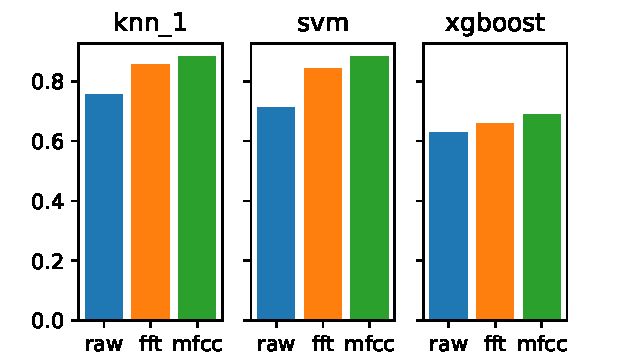
\includegraphics[width=0.7\textwidth]{figures/plots/model_comparison/custom_knn_1_xgboost_svm_main.pdf}
    \caption{Same preprocessing ranking between 1-NN, SVM and XGBoost on the Main dataset}
    \label{fig:selective_model_comparison_knn_xgboost_svm_main}
\end{figure}

\begin{figure}
    \centering
    \begin{subfigure}[b]{0.49\textwidth}
        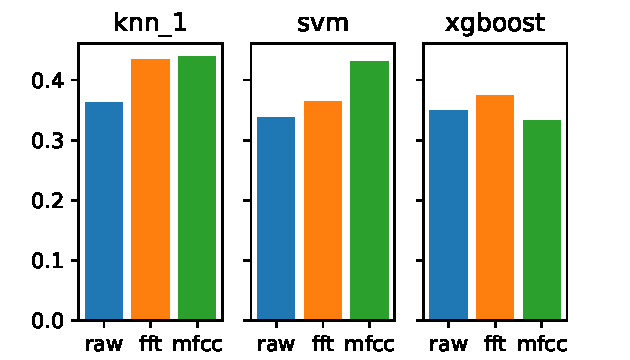
\includegraphics[width=\textwidth]{figures/plots/model_comparison/custom_knn_1_xgboost_svm_g213.pdf}
        \caption{G213}
        \label{fig:selective_model_comparison_knn_xgboost_svm_g213}
    \end{subfigure}
    \begin{subfigure}[b]{0.49\textwidth}
        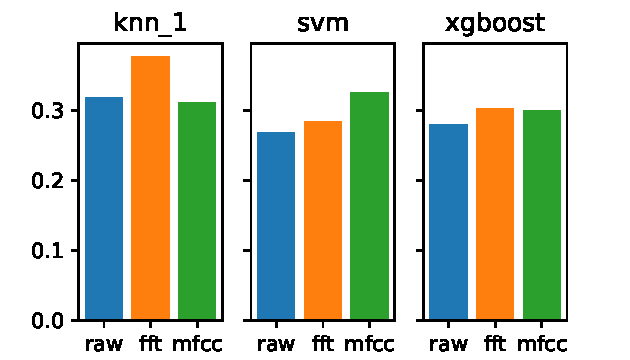
\includegraphics[width=\textwidth]{figures/plots/model_comparison/custom_knn_1_xgboost_svm_matebook14.pdf}
        \caption{MateBook14}
        \label{fig:selective_model_comparison_knn_xgboost_svm_matebook14}
    \end{subfigure}
    \caption{Clashing preprocessing rankings between 1-NN, SVM and XGBoost}
\end{figure}

\subsubsection{Logistic Regression, RNN}
A similar relationship was also observed for Logistic Regression and RNN. They
had the same preprocessing ranking and very similar accuracies on 4 out of 6
datasets (example illustrated on Figure~\ref{fig:selective_model_comparison_logistic_regression_rnn_main}).
Much like with the previous 3 models, one of the clashing datasets happened to be
MateBook14 (Figure~\ref{fig:selective_model_comparison_logistic_regression_rnn_matebook14}),
but this time the other one was
K3P (Figure~\ref{fig:selective_model_comparison_logistic_regression_rnn_k3p}).
\begin{figure}
    \centering
    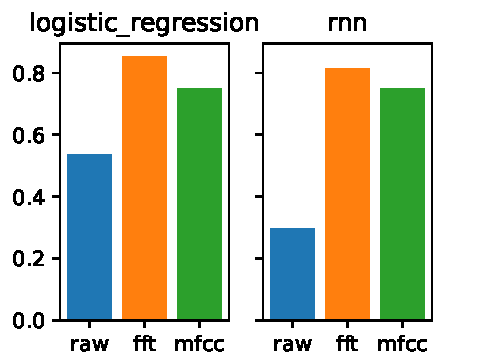
\includegraphics[width=0.5\textwidth]{figures/plots/model_comparison/custom_logistic_regression_rnn_main.pdf}
    \caption{Same preprocessing ranking between LR and RNN on the Main dataset}
    \label{fig:selective_model_comparison_logistic_regression_rnn_main}
\end{figure}

\begin{figure}
    \centering
    \begin{subfigure}[b]{0.49\textwidth}
        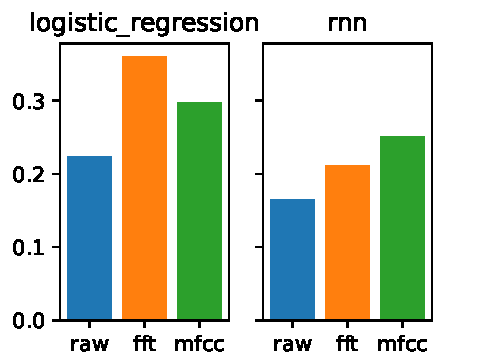
\includegraphics[width=\textwidth]{figures/plots/model_comparison/custom_logistic_regression_rnn_matebook14.pdf}
        \caption{MateBook14}
        \label{fig:selective_model_comparison_logistic_regression_rnn_matebook14}
    \end{subfigure}
    \begin{subfigure}[b]{0.49\textwidth}
        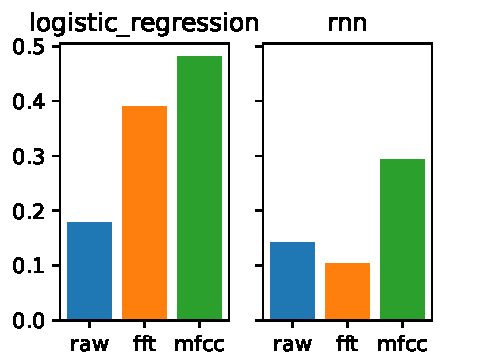
\includegraphics[width=\textwidth]{figures/plots/model_comparison/custom_logistic_regression_rnn_k3p.pdf}
        \caption{K3P}
        \label{fig:selective_model_comparison_logistic_regression_rnn_k3p}
    \end{subfigure}
    \caption{Clashing preprocessing rankings between LR and RNN}
\end{figure}

% MG TODO: is the order of paragraphs intentional here? It breaks the convention of alphabetical ordering 
\paragraph{MateBook14}
On MateBook14, RNN scored the highest with MFCC, followed by FFT and raw data in rather evenly-spaced intervals (25.1\%, 21.1\%, 16.5\%). On the contrary, Logistic Regression lead with FFT, followed by MFCC, and then raw data (36\%, 29.7\%, 22.3\%). Once again, the intervals are very even, but it is not an uncommon pattern to see in other models as well, so it seems there are no decisive or useful conclusions to be drawn here, aside from the fact that MateBook14 has proven its pattern-defying abilities for the second time.

\paragraph{K3P}
On K3P, the differentiating factor between both models was FFT, on which Logistic Regression performed relatively well (39\%), taking the middle spot between the best, MFCC, and the worst, raw data. On the other hand, RNN's results for FFT were quite terrible (10.5\%), putting it at the last spot below even raw data. What is interesting here is how Logistic Regression was the only model (out of all six types) to exhibit such a huge (21.2\%, or 91 examples) advantage of FFT over raw data on the K3P dataset. In all other cases, including RNN, the performances on FFT and raw data fell within a comparable range.

\subsubsection{Naive Bayes, SVM}
Naive Bayes did not match particularly well with any other model. A weak argument could be made for SVM, with which it technically agrees on 4 out of 6 datasets (exceptions being K3P and Main, as seen in Figure~\ref{fig:selective_model_comparison_naive_bayes_svm}). However, very often, SVM's middle-ranked preprocessing technique is roughly in the middle between first and last place. In contrast, Naive Bayes's middle- and last-ranked techniques are very close, making the order less clear and the shape of the ranking visibly different (Figure~\ref{fig:selective_model_comparison_naive_bayes_svm_CA_tb14}).
This property of 2nd and 3rd place forming a cluster was exhibited by all of Naive Bayes's rankings, with the sole exception of Main, where FFT and raw data were slightly more disjoint (by 10.2\%, or 44 examples, as seen in Figure~\ref{fig:selective_model_comparison_naive_bayes_svm_main}).

\begin{figure}
    \centering
    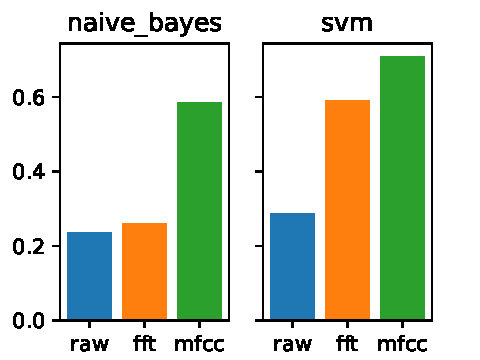
\includegraphics[width=0.5\textwidth]{figures/plots/model_comparison/custom_naive_bayes_svm_CA_tb14.pdf}
    \caption{Same preprocessing ranking between NB and SVM on the CA\_tb14 dataset}
    \label{fig:selective_model_comparison_naive_bayes_svm_CA_tb14}
\end{figure}

\begin{figure}
    \centering
    \begin{subfigure}[b]{0.49\textwidth}
        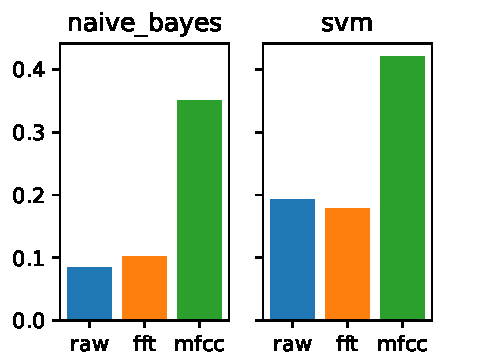
\includegraphics[width=\textwidth]{figures/plots/model_comparison/custom_naive_bayes_svm_k3p.pdf}
        \caption{K3P}
        \label{fig:selective_model_comparison_naive_bayes_svm_k3p}
    \end{subfigure}
    \begin{subfigure}[b]{0.49\textwidth}
        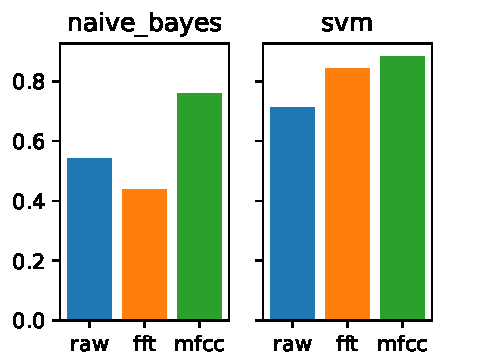
\includegraphics[width=\textwidth]{figures/plots/model_comparison/custom_naive_bayes_svm_main.pdf}
        \caption{Main}
        \label{fig:selective_model_comparison_naive_bayes_svm_main}
    \end{subfigure}
    \caption{Clashing preprocessing rankings between NB and SVM}
    \label{fig:selective_model_comparison_naive_bayes_svm}
\end{figure}

This is also a good place to mention that sharing preprocessing rankings is not a transitive relationship; despite Naive Bayes's vague similarity to SVM, it shares virtually none with 1-NN and XGBoost, despite both of them also being similar to SVM.

\section{Individual model performance} % discuss how different preprocessing techniques impact a model's performance
\label{sec:results_individual_model_performance}
\newcommand{\plotmodelsummary}[2]{%
\begin{figure}[H]%
    \centering%
    \includegraphics[width=0.8\textwidth]{figures/plots/model_summary/#1.pdf}%
    \caption{All accuracies achieved by #1 across datasets, peak types, and preprocessing techniques}
    \label{#2}%
\end{figure}%
}%

The focus of this section is to inspect the results of each model, how different preprocessing and peaks influence their performance, and to point out interesting observations. 

All considered models behaved differently based on applied preprocessing techniques, but most of them tended to prefer one technique over the other. Nevertheless, the chosen dataset also had an impact on the preferred preprocessing technique.

\subsection{1-NN}
1-NN achieved some of the best results in the experiments. It is worth mentioning that this model achieved decent accuracies of around 50\% for the "all" dataset, significantly higher than some of its peers.
This model did not have any particular preference for preprocessing (except on K3P, see \ref{sec:results_K3P}), whereas 4/6 models had a tendency to get better (or worse) results using one technique. 
The best three accuracies were achieved for dataset Main, with MFCC/\peaks{thr}, FFT/\peaks{th}, and FFT/\peaks{thr}, in that order.

\subsection{Logistic Regression}
Logistic Regression was consistently seen in the top 3 for all datasets, except Main and "all". For Main it achieved very good results, just slightly inferior to some other models. It is very frequently seen high in rankings of datasets that were of less quality than the Main dataset. Regarding the "all" dataset, it had better results than Naive Bayes, but it cannot be said that they were subpar compared to what one could expect given Logistic Regression's other performances. In the best scenario on this dataset, it passed 30\%, but that was significantly worse than what 1-NN and SVM achieved.

In the case of preprocessing, FFT was in favor of Logistic Regression (except K3P, \ref{sec:results_K3P}). Worse, but not necessarily bad, performance was achieved for MFCC. Using raw decreased accuracy even more. In most cases, raw preprocessing lowered results by more than 10 percentage points in comparison to FFT. 

The best 3 accuracies were achieved for the Main dataset, FFT, and peaks: \peaks{thr}, \peaks{th}, \peaks{tr}.

\subsection{Naive Bayes}
Naive Bayes is very interesting because of its extreme preference for MFCC preprocessing. Of 42 combinations of training datasets and peak sets, only once MFCC was worse than the other two. (it was for CA\_tb14 dataset and \peaks{t}, which is a strange situation in itself, \ref{sec:results_CA_tb14}) Also, the difference between MFCC and raw/FFT results is consistent and quite large, reliably getting an increase from 20 to even 50 percentage points increase in accuracy.

Overall, this model handled the "all" dataset worse than any other model, always scoring below 20\%. Except for the Main dataset and a few peaks/preprocessing combinations in CA\_tb14, the model did not pass 40\% accuracy.

The best three accuracies were achieved for dataset Main, MFCC preprocessing and peaks \peaks{thr}, \peaks{th}, \peaks{tr} in that order.

\subsection{Recurrent Neural Network}
This model had very similar results to Linear Regression but was slightly inferior to it. 

It usually got better accuracies for FFT, but for K3P, MateBook14, and part of G213, MFCC got better results. Another similarity to Linear Regression is that for most cases, raw preprocessing is worse than the other two, but to an even higher degree. It can be seen in the case of Main dataset, where the drop between FFT/\peaks{thr} and raw/\peaks{thr} is over 50\%. A comparison between performances on different datasets using all peak types and preprocessing techniques can be found in Figure~\ref{fig:rnn}

The best three accuracies were achieved for the Main dataset, FFT preprocessing and peaks \peaks{thr}, \peaks{th}, \peaks{tr} in that order.

Table~\ref{tab:results_rnn_main_top3} presents the predictions of RNN trained and tested on Main, using FFT preprocessing and \peaks{thr} peaks. The numbers represent how many times the sound of the corresponding key was found to be the first, second, and third most likely (in this order) by the network. For example, \verb|i| was never identified within the top three predictions, \verb|e| was correctly proposed four times as the most likely key, twice as the second and third each, while \verb|/| was always classified correctly. Table~\ref{tab:results_rnn_main_top3} was created to give a broader overview of the tendencies of the RNN, and to allow for a comparison with very similar tables found in "Keyboard Acoustic Emanations" \cite{og2004}, showcasing the predictions of the Artificial Neural Network developed therein. To facilitate a more direct comparison, the experiment configuration (preprocessing, peak type, and dataset) was selected to be the most similar to the ones found in the paper. 

% TABLE HERE, .csv on Discord
% DONE: PK
% done but unverified MG: adjust caption/label and the first table header row
%      also consider adding a paragraph explaining how to read the table
\newcommand{\tp}[3]{{\footnotesize #1,#2,#3}}
\begin{table}[h]
    \centering
    \caption{Number of correct top-3 recommendations for each of the keys during testing. The test set contained 10 presses of each key}
    \label{tab:results_rnn_main_top3}
    \begin{small}\textbf{}
    \begin{tabular}{|l|c|c|c|c|c|c|c|c|c|c|c|}
        \hline
        \multicolumn{12}{|c|}{\textbf{RNN with \peaks{thr} and FFT on dataset Main}} \\
        \hline
        \hline
        key pressed & 1 & 2 & 3 & 4 & 5 & 6 & 7 & 8 & 9 & 0 & - \\
        recognized & \tp{10}{0}{0} & \tp{10}{0}{0} & \tp{6}{0}{1} & \tp{10}{0}{0} & \tp{10}{0}{0} & \tp{10}{0}{0} & \tp{8}{0}{1} & \tp{8}{0}{0} & \tp{9}{0}{0} & \tp{10}{0}{0} & \tp{5}{3}{0} \\
        \hline
        \hline
        key pressed & q & w & e & r & t & y & u & i & o & p & \\
        recognized & \tp{5}{1}{0} & \tp{10}{0}{0} & \tp{4}{2}{2} & \tp{10}{0}{0} & \tp{8}{1}{0} & \tp{9}{1}{0} & \tp{6}{1}{1} & \tp{0}{0}{0} & \tp{9}{0}{0} & \tp{7}{1}{0} & \\
        \hline
        \hline
        key pressed & a & s & d & f & g & h & j & k & l & ; & ' \\
        recognized & \tp{7}{3}{0} & \tp{10}{0}{0} & \tp{9}{0}{0} & \tp{8}{1}{0} & \tp{7}{1}{0} & \tp{9}{0}{0} & \tp{0}{0}{0} & \tp{8}{0}{1} & \tp{10}{0}{0} & \tp{7}{2}{0} & \tp{9}{1}{0} \\
        \hline
        \hline
        key pressed & z & x & c & v & b & n & m & , & . & / & \\
        recognized & \tp{8}{0}{0} & \tp{10}{0}{0} & \tp{8}{1}{0} & \tp{9}{1}{0} & \tp{9}{1}{0} & \tp{9}{0}{0} & \tp{9}{0}{0} & \tp{10}{0}{0} & \tp{10}{0}{0} & \tp{10}{0}{0} & \\
        \hline
        \hline
        key pressed & \multicolumn{11}{|c|}{space} \\
        recognized & \multicolumn{11}{|c|}{\tp{10}{0}{0}} \\
        \hline
    \end{tabular}
    \end{small}
\end{table}
\let\tp\undefined

\plotmodelsummary{rnn}{fig:rnn}


\subsection{Support vector machines}
SVM achieves accuracies that are close to 1-NN results. On Main it breaks 80\% with several peak/preprocessing combinations. It also reaches second place in best accuracies for "all" dataset, which suggests that this model performs well in the case of datasets that contain more than one keyboard. 

Regarding preprocessing -- for this model, there are situations when the chosen technique does not change the accuracy by more than a few percent. At the same time, for the majority of cases, this model prefers MFCC preprocessing, while using raw preprocessing leads to a decrease in the quality of the model.

The 3 best accuracies were achieved for Main dataset, MFCC/\peaks{thr}, MFCC/\peaks{th} and FFT/\peaks{thr}

\subsection{XGBoost}
XGBoost behaved similarly to 1-NN in the regard that no preprocessing stood out from the rest (even for the K3P dataset, \ref{sec:results_K3P}). It did not perform terribly, but it was typically outshined by other models. 

What is also interesting about XGBoost, is that adding more peaks improved this model the least. For almost all model types and datasets (CA\_tb14 is an exception, \ref{sec:results_CA_tb14}). There was a slight tendency that the more peaks were included in the input, the better accuracies were achieved. Results of XGBoost show it loses the least information when fewer peaks are available (see Figure~\ref{fig:xgboost}. 

The best three accuracies were achieved for the Main dataset, MFCC preprocessing and peaks \peaks{thr}, \peaks{th}, \peaks{tr} (FFT/\peaks{thr} ties with 3rd accuracy) in that order. 

\plotmodelsummary{xgboost}{fig:xgboost}

%- across all the models fft/mfcc is better than none prep
% - all models prefer some kind of preprocessing
%    - rnn --> mfcc/fft,
%    - svm --> mfcc,
%    - xgboost --> almost no changes to prep, none slightly inferior
%    - 1-nn --> a little bit more than no changes to prep,


\end{document}